\documentclass[crop, tikz]{standalone}
\usepackage{tikz}

\usetikzlibrary{decorations.pathmorphing}

\definecolor{bluport}{HTML}{21ADFD}
\definecolor{orgport}{HTML}{E37322}
\definecolor{pplport}{HTML}{4F21E9}
\definecolor{redport}{HTML}{701315}

\begin{document}
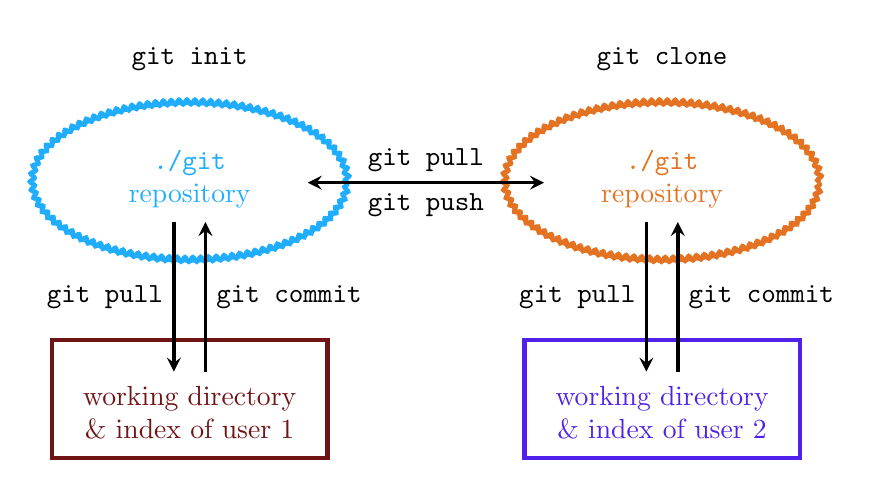
\begin{tikzpicture}
	\draw[thick, bluport] (0, 0) ellipse (2 and 1);
	\draw[ultra thick, bluport, decorate, decoration={snake, segment length=1mm, amplitude=0.3mm}] (0, 0) ellipse (2 and 1);
	\node[text height=1em, text depth=1em] (1) at (0, 1.5) {\tt git init};
	\node[text height=1em, text depth=1em, align=center, bluport] (1) at (0, -0.25) {\tt ./git \\ repository};
		
	\draw[thick, orgport] (6, 0) ellipse (2 and 1);
	\draw[ultra thick, orgport, decorate, decoration={snake, segment length=1mm, amplitude=0.3mm}] (6, 0) ellipse (2 and 1);
	\node[text height=1em, text depth=1em] (1) at (6, 1.5) {\tt git clone};
	\node[text height=1em, text depth=1em, align=center, orgport] (1) at (6, -0.25) {\tt ./git \\ repository};
		
	\draw[ultra thick, redport] (-1.75, -2) rectangle (1.75, -3.5);
	\node[text height=1em, text depth=1em, align=center, redport] (1) at (0, -3.25) {working directory \\ \& index of user 1};
		
	\draw[ultra thick, pplport] (4.25, -2) rectangle (7.75, -3.5);
	\node[text height=1em, text depth=1em, align=center, pplport] (1) at (6, -3.25) {working directory \\ \& index of user 2};
		
	\draw[very thick, stealth-stealth] (1.5, 0) -- node[above] {\tt git pull} node[below] {\tt git push} (4.5, 0);
		
	\draw[very thick, -stealth] (-0.2, -0.5) -- node[left] {\tt git pull} (-0.2, -2.4);
	\draw[very thick, -stealth] (0.2, -2.4) -- node[right] {\tt git commit} (0.2, -0.5);
		
	\draw[very thick, -stealth] (5.8, -0.5) -- node[left] {\tt git pull} (5.8, -2.4);
	\draw[very thick, -stealth] (6.2, -2.4) -- node[right] {\tt git commit} (6.2, -0.5);
\end{tikzpicture}
\end{document}